\section{Appendix}
%\setcounter{section}{0}
%\setcounter{subsection}{0}

\subsection{The Properties of the Learned Latent Space}
\label{ch3:sec:discussion}

\subsubsection{The Smoothness of Latent Space}
We analyze the latent space's smoothness by interpolating the latent codes of two different airfoils $\bz_1$ and $\bz_2$.
The interpolated $M^S$ is extracted from the reconstructed CFD mesh decoded from a weighted sum of $z_1$ and $z_2$, namely $M(\hat{\bv} + g_{\Theta}(w_1\bz_1 + w_2\bz_2))$, where $w_1\in (0,1)$ and $w_2=1-w_1$ are interpolation weights.
We select some visually distinguishable airfoils and show the interpolated results in Fig.\ref{ch3:fig:discuss_latent_interp}, which included interpolations within NACA airfoils, non-NACA airfoils and between different airfoil series.
Each row in Fig.\ref{ch3:fig:discuss_latent_interp} shows a gradual transformation on shape, indicating the change of $w_1\bz_1 + w_2\bz_2$ in the latent space is also smooth.

\begin{figure}[!htb]
	\begin{center}
		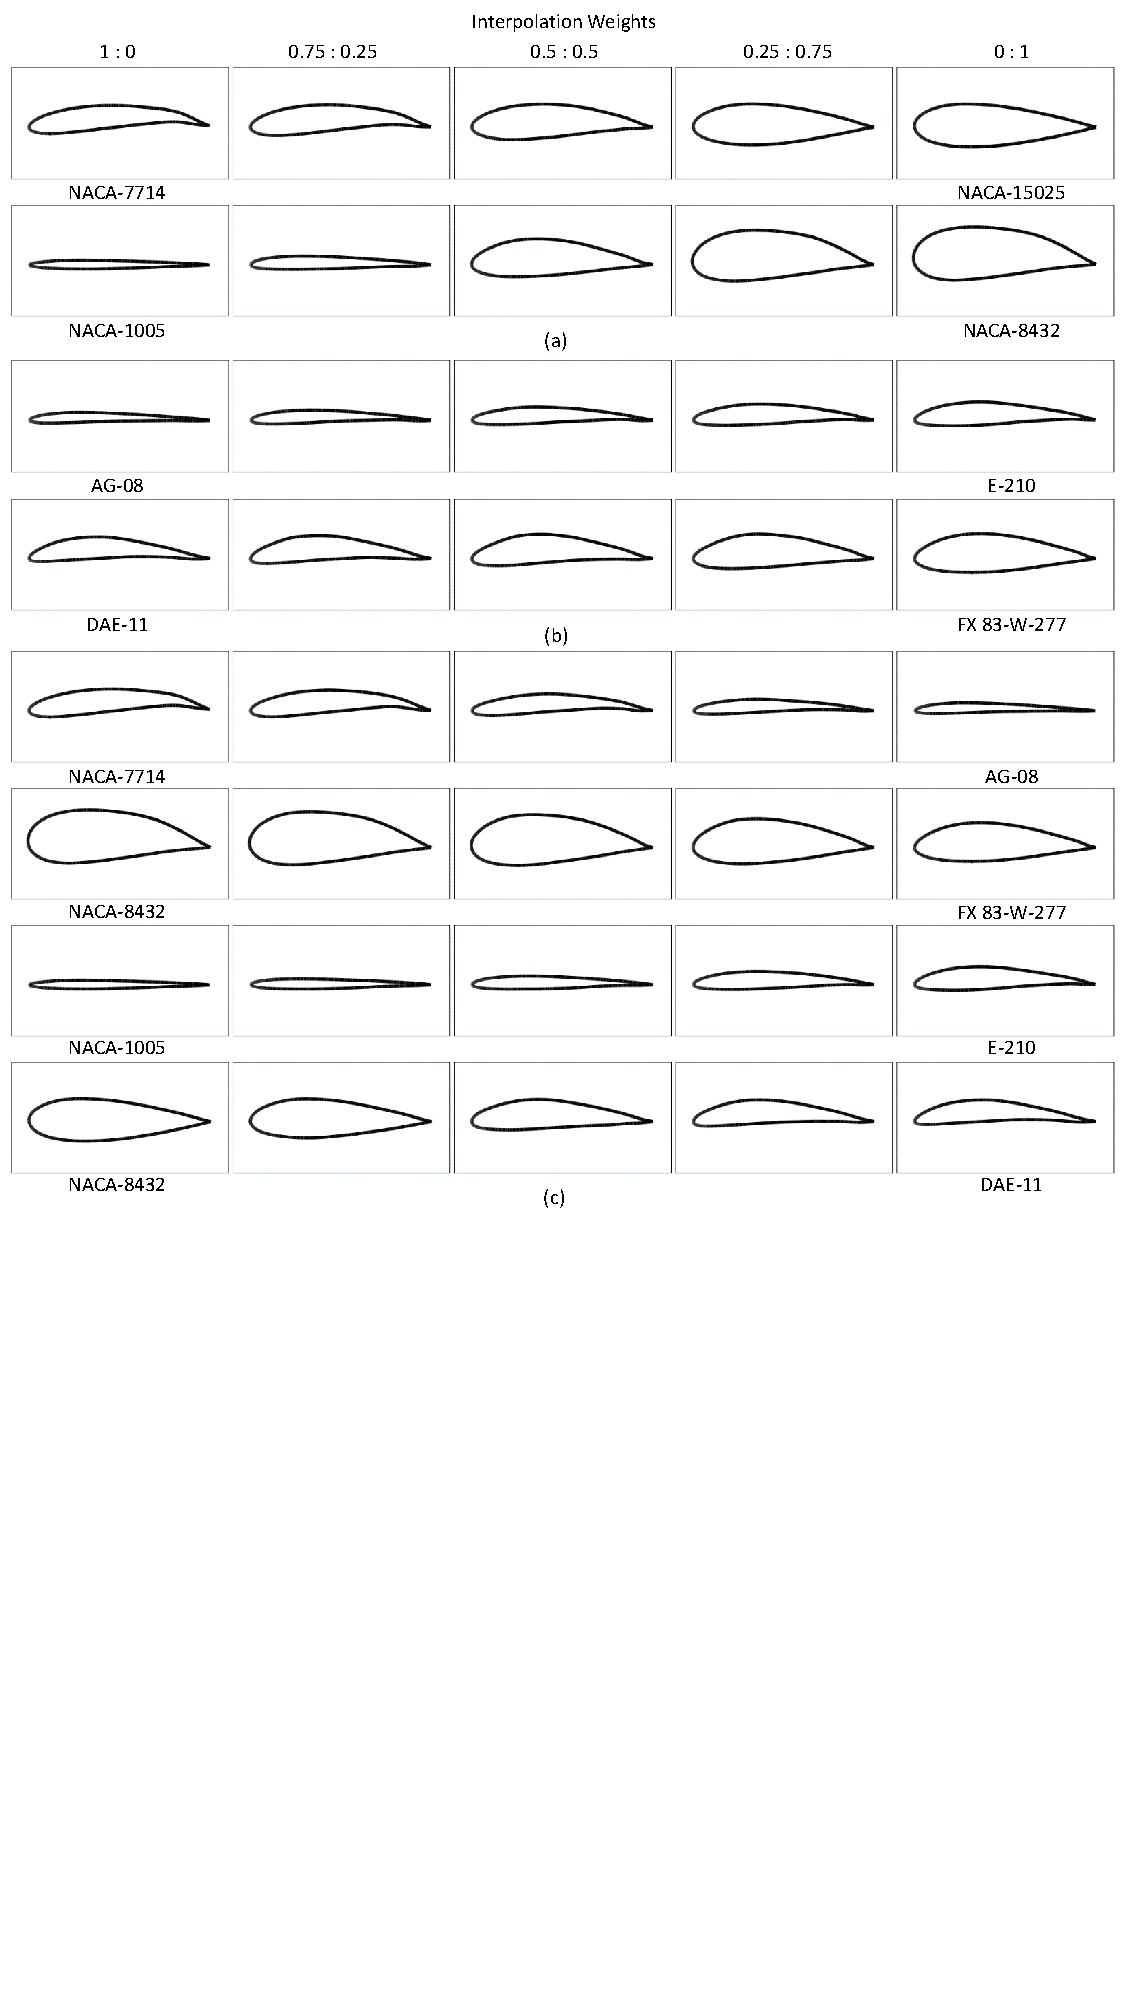
\includegraphics[width=1\linewidth]{chapter3/tex/figures/experiment/latent_interpolation.pdf}
	\end{center}
	\caption{
		\small Decoded airfoils by interpolating between latent codes of (a) NACA, (b) non-NACA and (c) mixed airfoils.
	}
	\label{ch3:fig:discuss_latent_interp}
\end{figure}


\subsubsection{The Learned Geometric Patterns}
Here we visualize the learned geometric patterns by analysing the latent space's principle components (PC).
Instead of collecting many latent codes, performing SVD and then computing the PCs, we follow a sampling-free approach \cite{ai.Shen2021b} to decompose the latent space. We modify it to apply it on the auto-decoder model.
The first layer of auto-decoder is a graph convolution where the node features are the coordinate of $\hat{\bv}_i$ and latent code $\bz$. The feature it extracts $f_1$ is
\begin{equation}
    f_1 = \sigma(\sum_i^N\Theta_1 [\hat{\bv}_i, \bz])\;,
\end{equation}
where $\sigma(.)$ is the activation function, $\Theta_1$ is the first layer parameter in $g_\Theta$, $N$ means $N$ neighboring vertices connected to $\hat{\bv}_i$ and $[.,.]$ means vector concatenation.
This process can be equally written as
\begin{equation}
    f_1 = \sigma(\sum_i^N(\Theta_{1;v}\hat{\bv}_i + \Theta_{1;z} \bz))\\;,
\end{equation}
where $\Theta_{1,v}$ and $\Theta_{1,z}$ are split from $\Theta_1$.
Then the principle components are calculated from the matrix decomposition of $(\Theta_{1,z}^T \Theta_{1,z})$.

\begin{figure}[!htb]
	\begin{center}
		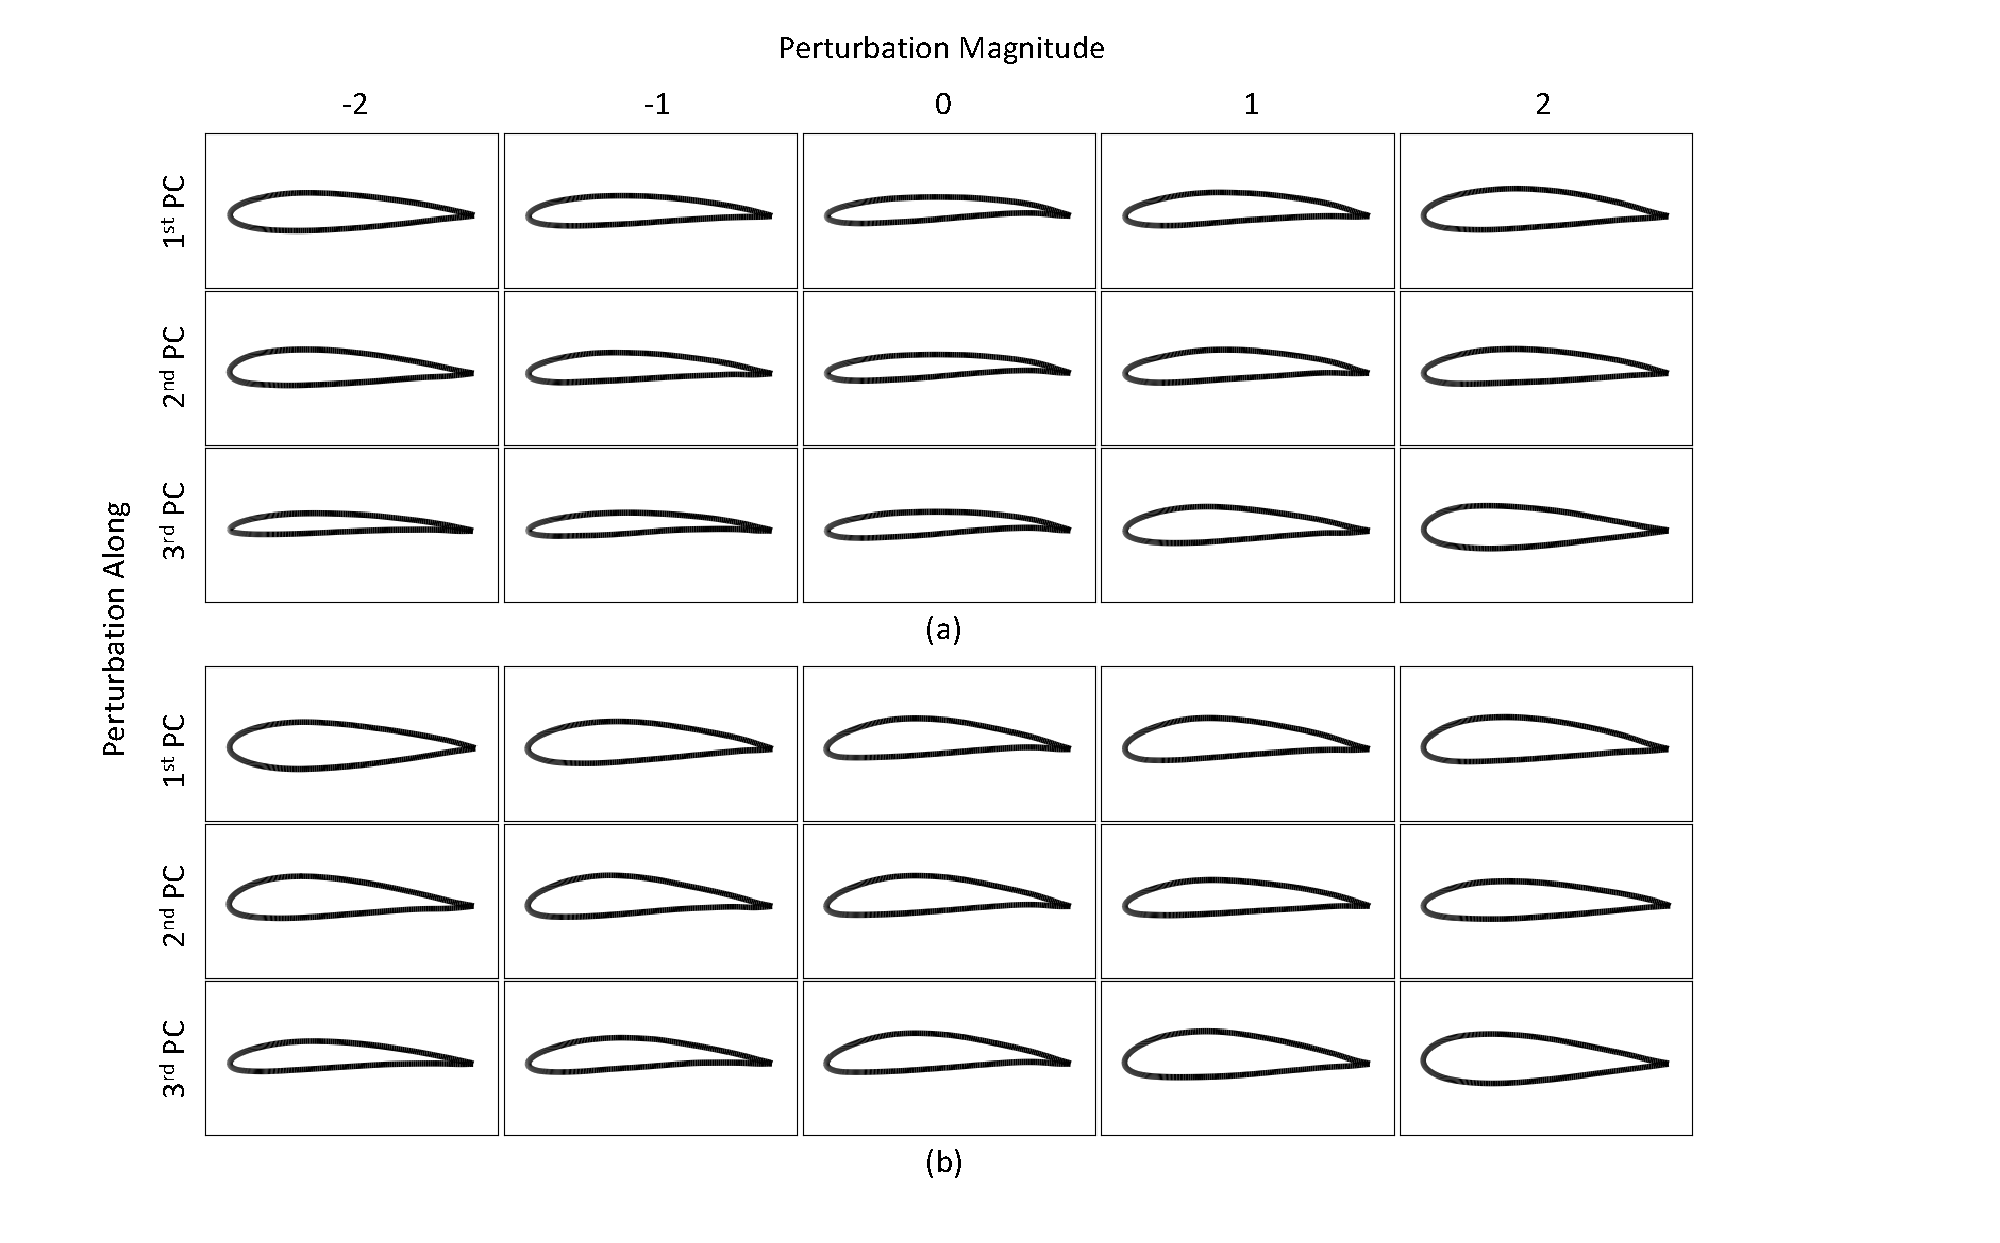
\includegraphics[width=1\linewidth]{chapter3/tex/figures/experiment/latent_factorization.pdf}
	\end{center}
	\caption{
		\small Decoded airfoils by perturbing the top 3 PCs from (a) NACA-4710's and (b) LA203A's latent codes.
	}
	\label{ch3:fig:discuss_latent_factor}
\end{figure}
\begin{figure}[!htb]
	\begin{center}
		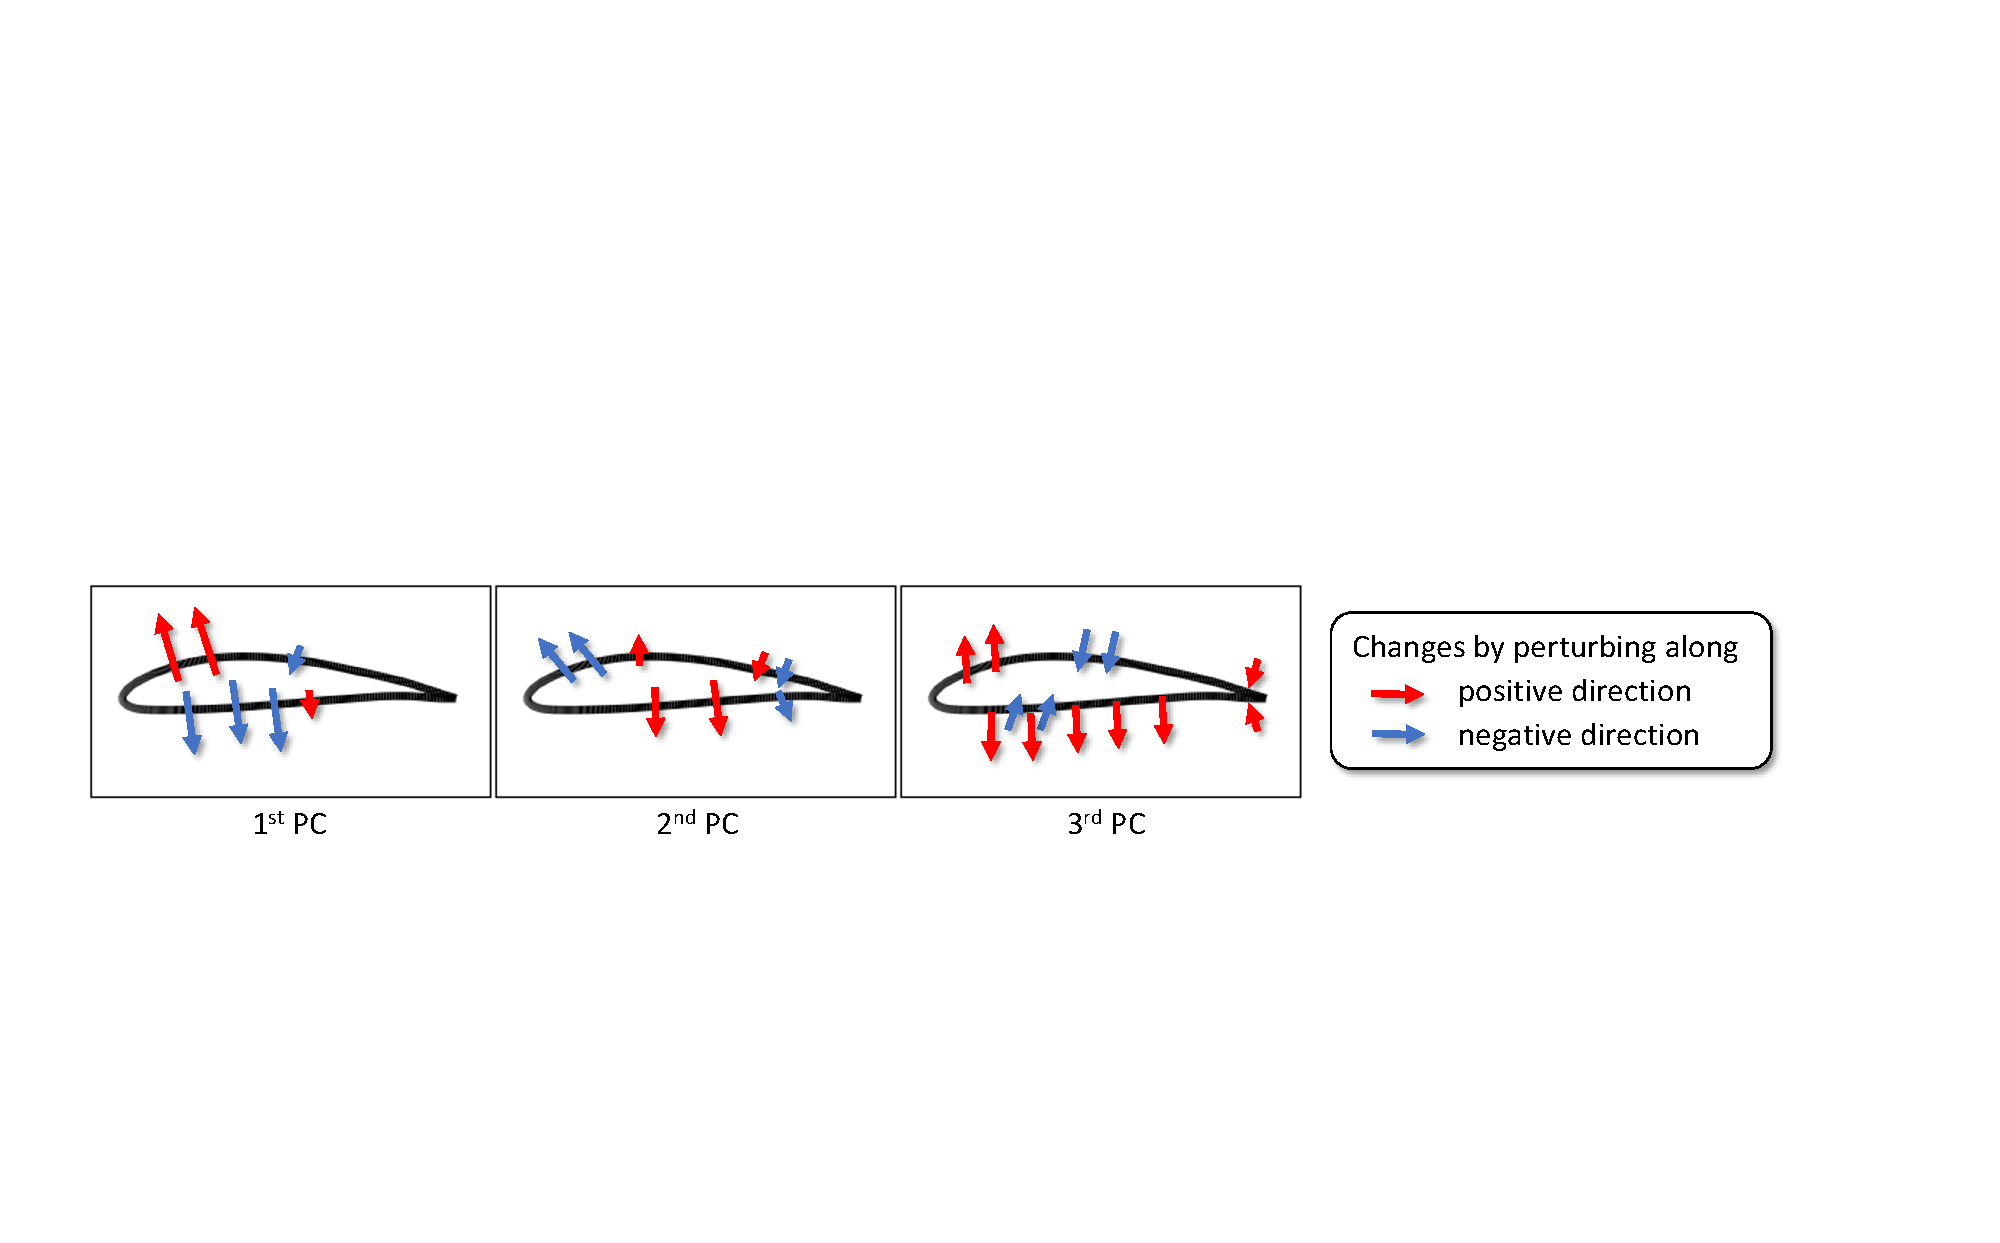
\includegraphics[width=1\linewidth]{chapter3/tex/figures/experiment/latent_factorization_pattern.pdf}
	\end{center}
	\caption{
		\small Visualized top 3 PCs. Arrows represent changes by perturbing PCs along different directions.
	}
	\label{ch3:fig:discuss_latent_factor_pattern}
\end{figure}

In Fig.\ref{ch3:fig:discuss_latent_factor}, we demonstrate the explored novel shapes by perturbing the latent codes of existing airfoils along the directions of top 3 PCs.
All novel shapes have noticeable changes.
We can observe common patterns for each PC.
For example, when perturbing along the first PC, the shapes extend upward at the leading edges while the shapes bulge downward with the negative perturbations.
Fig.\ref{ch3:fig:discuss_latent_factor_pattern} shows the learned patterns of the top three PCs.
These observations indicate that the latent space has discovered and acquired geometric prior knowledge via learning.

\subsection{Calculating Finite Difference Approximation}
\label{ch3:sec:appendix_finite_difference}
Since the following explanation is the same for all vertices and combinations of neighbors, we omit the subscripts $i$ and $b$ for simplicity.

The definition of $\mathbf{r}$, $\bt$ and the sampling strategy of $\Delta\mathbf{r}^+$, $\Delta\mathbf{r}^-$, $\delta\mathbf{t}^+$ and $\Delta\mathbf{t}^-$ are described in Sec.\ref{ch3:sec:loss} and illustrated in Fig.\ref{ch3:fig:coords}.
The subscript $i$ is omitted for simplicity. 
Let's denote the finite difference sampling, e.g. on axis $\mathbf{r}$, as
\begin{align*}
    & \bv(r + \Delta {r^ + },t) = r\mathbf{r} + \Delta \mathbf{r}^ + + t\mathbf{t}\;, \cr
    & \bv(r - \Delta {r^ - },t) = r\mathbf{r} + \Delta \mathbf{r}^ - + t\mathbf{t}\;.
\end{align*}
Then the finite difference approximations for the derivatives in Eq.\ref{ch3:eq:euler_lagrange} can be written as
\begin{align*}
  & \frac{{\partial \bv}}{{\partial r}} \approx \frac{1}{{\Delta r}}[\bv(r + \Delta {r^ + },t) - \bv(r,t)]\;,  \cr 
  & \frac{{{\partial ^2}\bv}}{{\partial {r^2}}} \approx \frac{1}{{\Delta {r^2}}}[\bv(r + \Delta {r^ + },t) - 2\bv(r,t) + \bv(r - \Delta {r^ - },t)]\;,  \cr 
  & \frac{{{\partial ^4}\bv}}{{\partial {r^4}}} \approx \frac{1}{{\Delta {r^4}}}[\bv(r + 2\Delta {r^ + },t) - 4\bv(r + \Delta {r^ + },t) + 6\bv(r,t) - 4\bv(r - \Delta {r^ - },t) + \bv(r - 2\Delta {r^ - },t)]\;.
\end{align*}
Similarly, we can write the finite difference approximation w.r.t. $t$ as well.

\subsection{Proof of Validity of Sampling Strategy}
\label{ch3:sec:appendix_sampling_proof}
Similar as in Appendix.B, we omit the subscript $b$ for simplicity.

In Sec.\ref{ch3:sec:loss} and Eq.\ref{ch3:eq:delta_r_t}, we propose how to sample perturbations to approximate the derivatives in Eq.\ref{ch3:eq:euler_lagrange}.
This is different from the standard definition to compute a derivative and we give a proof to show why such a sampling method can be an approximation.
First, we use a term $l(r_i, t_i)$, a function of vertex $\bv_i(r_i,t_i)$, as a concise substitute of $g_\Theta(\bz, M)$ when the latent code, edges and vertices except for $\bv_i$ in $M$ are fixed.
In this case, we can write $\mathbf{dv}_i=l(r_i, t_i)$ and $\bv_i=\mathbf{\hat{v}}_i+l(r_i, t_i)$.

In theory, the finite difference of $\bv_i$ should be written as
\begin{align*}
    \bv_i(r_i + \Delta r,t_i) 
    &= (r_i + \Delta r)\mathbf{r}_i + t_i\bt_i + l(r_i + \Delta r,t_i) \\
    &= {r_i}{\mathbf{r}_i} + {t_i}{\bt_i} + \Delta r{\mathbf{r}_i} + l({r_i} + \Delta r,{t_i}) \\
    &= {\hat{\bv}_i} + \epsilon {\mathbf{r}_i} + l({r_i} + \Delta r,{t_i})\;,
\end{align*}
where the magnitude of perturbation $|\Delta r|=\epsilon$.
By expanding $l({r_i} + \Delta r,{t_i})$ with the first order Taylor expansion at $\hat{\bv}_i$, we have
\begin{align*}
    {\bv_i}({r_i} + \Delta r,{t_i}) 
    &= \hat{\bv}_i + \epsilon {\mathbf{r}_i} + l({r_i} + \Delta r,{t_i}) \\
    &= \hat{\bv}_i + \epsilon {\mathbf{r}_i} + l({r_i},{t_i}) + {{\partial l({r_i},{t_i})} \over {\partial r}} (\hat{\bv}_i + \Delta r \mathbf{r}_i - \hat{\bv}_i) + O({{{\partial ^2}l} \over {\partial {r^2}}}) \\
    &= \hat{\bv}_i + \epsilon {\mathbf{r}_i} + l({r_i},{t_i}) + {{\partial l({r_i},{t_i})} \over {\partial r}}(\epsilon {\mathbf{r}_i}) + O({{{\partial ^2}l} \over {\partial {r^2}}}) \\
    &\approx \hat{\bv}_i + \epsilon {\mathbf{r}_i} + l({r_i},{t_i}) + {{\partial l({r_i},{t_i})} \over {\partial r}}(\epsilon {\mathbf{r}_i}) \;.
\end{align*}
In practice, we use a different finite difference instead
\begin{align*}
     {\bv_i}({r_i},{t_i}) + \Delta {\mathbf{r}_i}^ +  
     &= \hat{\bv}_i + l({r_i},{t_i}) + \epsilon {( {\bv_{ir} - \bv_i} ) \over {||{\hat{\bv}_{ir}} - {\hat{\bv}_i}||^2} } \\
     &= \hat{\bv}_i + l({r_i},{t_i}) + \epsilon ({{{\hat{\bv}_{ir}} - {\hat{\bv}_i}} \over ||{\hat{\bv}_{ir}} - {\hat{\bv}_i}||^2} + {{l({r_{ir}},{t_{ir}}) - l({r_i},{t_i})} \over {||{\hat{\bv}_{ir}} - {\hat{\bv}_i}||^2}}) \\
     &= \hat{\bv}_i + l({r_i},{t_i}) + \epsilon \mathbf{r}_i + \epsilon {{l({r_{ir}},{t_{ir}}) - l({r_i},{t_i})} \over ||{\hat{\bv}_{ir}} - {\hat{\bv}_i}||^2} \;.
\end{align*}
Again, we use the first order Taylor expansion of $l({r_{ir}},{t_{ir}})$ at $\hat{\bv}_i$. Considering $\epsilon$ is a very small value, we have
\begin{align*}
    {\bv_i}({r_i},{t_i}) + \Delta {\mathbf{r}_i}^ +  
    &= \hat{\bv}_i + l({r_i},{t_i}) + \epsilon \mathbf{r}_i + \epsilon {{l({r_{ir}},{t_{ir}}) - l({r_i},{t_i})} \over {||{\hat{\bv}_{ir}} - {\hat{\bv}_i}||^2}} \\
    &= \hat{\bv}_i + l({r_i},{t_i}) + \epsilon \mathbf{r}_i + {{\partial l({r_i},{t_i})} \over {\partial r}}(\epsilon {\mathbf{r}_i}) + O(\epsilon^2 {{{\partial ^2}l} \over {\partial {r^2}}}) \\
    &\approx \hat{\bv}_i + l({r_i},{t_i}) + \epsilon \mathbf{r}_i + {{\partial l({r_i},{t_i})} \over {\partial r}}(\epsilon {\mathbf{r}_i}) \\
    &\approx {\bv_i}({r_i} + \Delta r,{t_i}) \;. 
    \;\;\;\;\square
\end{align*}

Similarly, we can write down the negative perturbation in theory as 
\begin{equation*}
    {\bv_i}({r_i} - \Delta r,{t_i}) \approx \hat{\bv}_i - \epsilon {\mathbf{r}_i} + l({r_i},{t_i}) - {{\partial l({r_i},{t_i})} \over {\partial r}}(\epsilon {\mathbf{r}_i})\;.
\end{equation*}
Let's define the affine transformation matrix $R(\alpha)$ that rotates $\mathbf{\Delta t}^+$ into $\mathbf{\Delta r}^-$ as $\mathbf{\Delta r}^- = R(\alpha)\mathbf{\Delta t}^+$.
Then we can write down the finite difference used in practice as
\begin{align*}
    {\bv_i}({r_i},{t_i}) + \Delta {\mathbf{r}_i}^ -  
    &= {\bv_i}({r_i},{t_i}) + R(\alpha )\Delta {\bt_i}^ + \\
    &= \hat{\bv}_i + l({r_i},{t_i}) + \epsilon R(\alpha ){{{\bv_{it}} - {\bv_i}} \over {||{\hat{\bv}_{it}} - {\hat{\bv}_i}|{|^2}}} \\
    &= \hat{\bv}_i + l({r_i},{t_i}) + \epsilon R(\alpha ){\bt_i} + \epsilon R(\alpha ) {{l({r_{it}},{t_{it}}) - l({r_i},{t_i})} \over {||{\hat{\bv}_{it}} - {\hat{\bv}_i}||^2}}\;.
\end{align*}
By use the first order Taylor expansion of $l({r_{it}},{t_{it}})$ at $\hat{\bv}_i$, we have
\begin{align*}
    {\bv_i}({r_i},{t_i}) + \Delta {\mathbf{r}_i}^ -  
    &= \hat{\bv}_i + l({r_i},{t_i}) + \epsilon R(\alpha ){\bt_i} + \epsilon R(\alpha ) {{l({r_{it}},{t_{it}}) - l({r_i},{t_i})} \over {||{\hat{\bv}_{it}} - {\hat{\bv}_i}||^2}} \\
    &\approx \hat{\bv}_i + l({r_i},{t_i}) + \epsilon R(\alpha ){\bt_i} + \epsilon R(\alpha ) {{\partial l({r_i},{t_i})} \over {\partial t}}{\mathbf{t}_i} \\
    &= \hat{\bv}_i - \epsilon {\mathbf{r}_i} + l({r_i},{t_i}) - {{\partial l({r_i},{t_i})} \over {\partial r}}(\epsilon {\mathbf{r}_i}) \\
    &\approx {\bv_i}({r_i} - \Delta r,{t_i}) \;.
    \;\;\;\;\square
\end{align*}

In conclusion, the vicinity of $\bv_i$ in the tangent space of $M$ at vertex $\bv_i$ is an approximation of the real manifold with first order accuracy. $\bv_i+\Delta \mathbf{r}_i^+$ and $\bv_i+\Delta \mathbf{r}_i^-$ can substitute $\bv_i(r_i+\Delta r, t_i)$ and $\bv_i(r_i-\Delta r, t_i)$, respectively.
Similar conclusions also apply for perturbations towards other directions.

\subsection{Details of Surrogate Based Optimization and Surrogate Model}
\label{ch3:sec:appendix_surrogate}

Our shape optimization followed the major procedures of the surrogate-based optimization (SBO) \cite{aa.Queipo2005}. The main steps are listed below.

\begin{algorithm}
    \caption{The workflow of our shape optimization.}
    \label{ch3:alg:RL-SBO}

    \textbf{Given:} Airfoils from the UIUC database and their RANS simulation results.

    1. Construct a GCNN surrogate model based on the RANS pressure data.

    2. Minimize the optimization objectives as defined in Eq.22.

    3. Sample optimized shapes generated from different initial airfoils, perform RANS simulations and update the surrogate model using new data.

    4. Minimize the optimization objectives again with the updated GCNN.
\end{algorithm}

More specifically, $1,000$ airfoils are collected at Step 1 and $300$ shapes are sampled at Step 3.

As for the surrogate model, the same network architecture of the surrogate model proposed in \cite{aa.Baque2018} is used.
The model is composed of 5 graph convolution blocks.
Each block contains 3 graph convolutional layers.
A batch normalization layer is used after each graph convolutional layers and the Exponential Linear Unit is used as the activation function.
The surrogate model takes $M^S$ as input.
It predicts the pressure value for each vertex and the drag coefficient can be computed via an integral on the airfoil's surface.
To train and update the surrogate model, the Adam optimizer is adopted with the learning rate as $5\times10^{-4}$. The training uses $900$ epochs.